\documentclass[]{article}
\usepackage{graphicx}
\usepackage{caption}
\usepackage{subcaption}
%opening
\title{ECE 657A Assignment \#2}
\author{Yuzhou Wang (20609396), Laura McCrackin (20262085), \newline and   Huang Tianhui (20587328)       }


\begin{document}

\maketitle


%%\begin{figure}
%\includegraphics{../images/741741}
%%\end{figure}

\section{Parameter Selection and Classification (for dataset D)}
Classify dataset D using five classifiers: k-NN, Support Vector Machine (with RBF kernel), Naïve Bayes Classifier, Decision Trees and Neural Networks. 
\subsection{question 1}
1)Preprocess the given data using the Z-score normalization, and split the data into two halves, the first half being the training set and the second half being the test set. (Normally you would do this randomly, but for this assignment a deterministic split will make the rest of the answers easier to grade).

For the original dataset D, we notice that there is no missing values, the value is around the average mean, so we could use Z-score normalization to separate the data into two groups and use the function “zscore” in Matlab library directly. Our group use the first half of data for training, the second for testing, and use the same split method for both gnd feature and given data.




\subsection{question 2}
2)For k-NN you need to evaluate the best value k to use. Using 5-fold cross validation (the crossvalind function can help) on the training set evaluate k-NN on the values k=[1, 3, 5, 7, ..., 31]. Plot a figure that shows the relationship between the accuracy and the parameter k. Report the best k in terms of classification accuracy.

For 5-fold cross validation, we could use the function "crossvalind", and use "fitcknn" to find K-NN neighbours. And for the calculation of accuracy, we could use "predict" function to judege the reality result is how similar with the therotical result. And insetead of the loop, everytimes we compare the best k, so that we could get the best K. For run time calculate, we could use "tic", "toc" function directly. By spliting data into training data and test data, and judge the result, we could get the truth positive, truth negarive, false positive and false negetive respectively. For more details, could refernce the code.


\begin{figure}[p]
	\centering
	\begin{subfigure}{.5\textwidth}
		\centering
		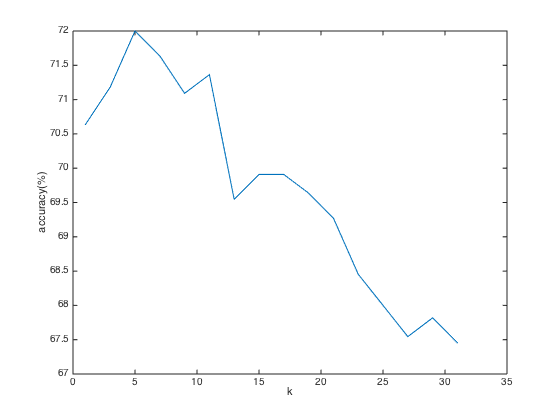
\includegraphics[width=1\linewidth]{../images-update/1-(2)-1.png}
		\caption{k=5}
		\label{fig:sub1}
	\end{subfigure}
	
	\begin{subfigure}{.5\textwidth}
		\centering
		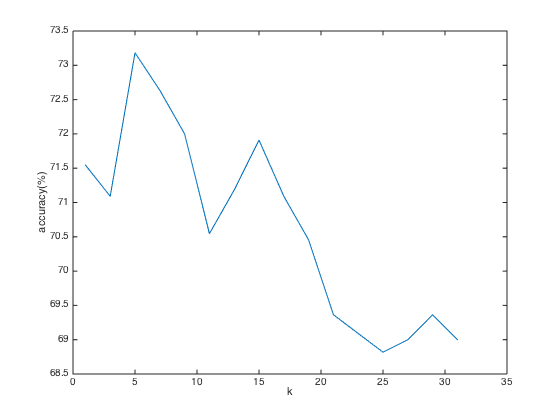
\includegraphics[width=1\linewidth]{../images-update/1-(2)-2.png}
		\caption{k=5}
		\label{fig:sub1}
	\end{subfigure}
	%\caption{Data histograms before normalization.}
	%\label{fig:hist1}
	
	\begin{subfigure}{.5\textwidth}
		\centering
		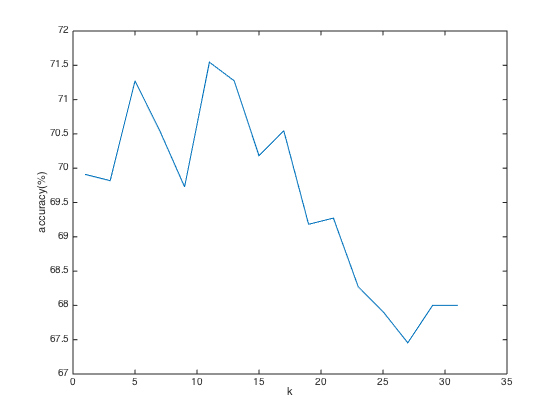
\includegraphics[width=1\linewidth]{../images-update/1-(2)-3.png}
		\caption{k=12}
		\label{fig:sub1}
	\end{subfigure}
	
	\begin{subfigure}{.5\textwidth}
		\centering
		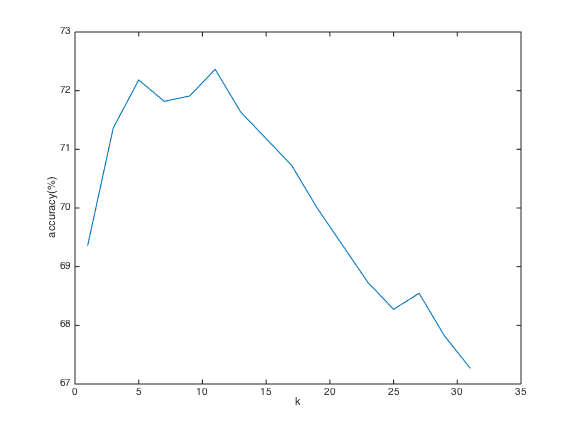
\includegraphics[width=1\linewidth]{../images-update/1-(2)-4.png}
		\caption{k=12}
		\label{fig:sub1}
	\end{subfigure}		
\end{figure}

Here we could see these two pictures for K-NN, and some different result could get. 
For the above four pictures, we could notice that everytime the best k changes, the value of best k is around 5-12 and the accuracy is between 71\% and 73\%.

We could also notice that when k is smaller than the range of best k, the accuracy increased and later larger the largest best k, it decreased. I think maybe it is the reason that less than k points is to small to be a class, in other words, less points can not represent a class, but if K is too large, then it means that some other classes's points maybe be included, which leads to a lower accuracy. Lastly, since we randomly choose the dataset and split them so that there could be some flexible results also.
And what is more, we should also notice about the accuracy about the dataset itself, maybe there are some outliers. And what is more, since it is DNA sequence, it means some cuts may represent nothing, but it still appears at the dataset with a label. Above all, the result we get maybe not the exactly right answer.




\subsubsection{question 3}
3)For the RBF kernel SVM, there are two parameters to be decided: the soft margin penalty term "c" and the kernel width parameter “gamma”. Again use 5-fold cross validation on the training set to select the parameter "c" from the set [0.1, 0.5, 1, 2, 5, 10, 20, 50] and select the parameter “gamma” from the set [0.01, 0.05, 0.1, 0.5, 1, 2, 5, 10]. Report the best parameters in terms of classification accuracy including plotting the ROC curves.



Since the purpose of SVM is to produce a classifier that will work well on unseen examples (generalizes well), so it belongs to the decision (function) boundary approach. For design details, we could use two "for" loops, we could generate different combinations of "c" and "gamma". Firstly, we use the "sprintf" function to deal with different c and gamma as input. Later use "libsvmtrain" to training the data, use "libsvmpredict" to predict the data, and for calculating the trueth positive part, similar with the above.

According to the best c and gamma, we could trace the ROC plot.C is the cost of classification as correctly stated, a large C gives you low bias and high variance. Low bias because you penalize the cost of missclasification a lot. A small C gives you higher bias and lower variance. Gamma is the parameter of a Gaussian Kernel (to handle non-linear classification). For non-linear classification, gamma controls the shape of the "peaks" where you raise the points. A small gamma gives you a pointed bump in the higher dimensions, a large gamma gives you a softer, broader bump.So a small gamma will give you low bias and high variance while a large gamma will give you higher bias and low variance. Theoretically with the increasing of gamma(kennel width), the accuracy decrease, because if the gamma is small enough(nearly 0), then it means that data point is not influenced or correlated with other data points. Small kernel width may cause over-fitting, and large one under-fitting. The so-called optimal kernel width is merely selected based on the tradeoff between under-fitting loss and over-fitting loss. 


\begin{figure}[p]
	\centering
	\begin{subfigure}{.5\textwidth}
		\centering
		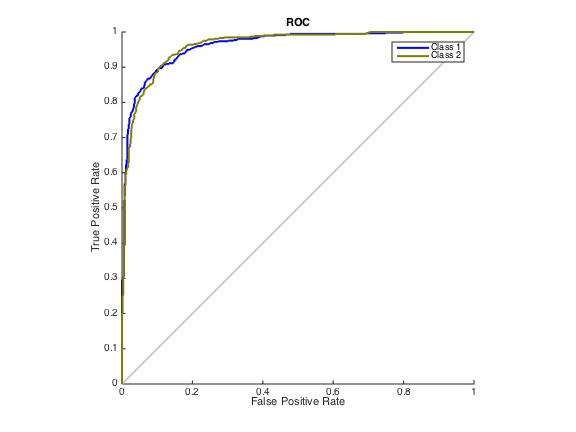
\includegraphics[width=1\linewidth]{../images-update/1-(3)-2.png}
		\caption{ROC}
		\label{fig:sub1}
	\end{subfigure}
		 
\end{figure}




\subsubsection{question 4}
4)Using the chosen parameters from the above parameter selection process for k-NN and SVM, and the default setups for Naive Bayes classifier, Decision Tree and Neural Network, classify the test set. Repeat each classification method 20 times by varying the split of training-test set (now select a random half of the data for training and the other half for test). Report the average and standard deviation of classification performance on the test set regarding: accuracy, precision, recall, and F- Measure. Also report the training time and classification time of the four methods.

Since we need to calculate the data result for 20 times, so define different matrix result and all the initial values are all 0. For Naive Bayes classifier function could use "fitNaiveBayes" function directly, the training process or calculate true positive are all similar to the above method. And for decision tree classifier could use function "fitctree" and method also similar to the above. For neural network, we could first create a neutal network by the function of patternnet and hidden layer by default is 10. For training method, we could use "train" function, and label different networks according to the test result, by setting and labelling class by hand, we could better compare with test set.

From the accuracy table above, we could see that the best method is decision tree with the highest accuracy, precision,recall and F-measure but it is also the waste most of time to decide. The worst answer result is from K-NN method.

For neural network, we could see the result in picture "perfomance".  Generally, the error reduces after more epochs of training, but might start to increase on the validation data set as the network starts overfitting the training data. In the default setup, the training stops after six consecutive increases in validation error, and the best performance is taken from the epoch with the lowest validation error. Next we could see figre "neural-confusion". Since result – outputs = targets. The R value is an indication of the relationship between the outputs and targets. If R = 1, this indicates that there is an exact linear relationship between outputs and targets. If R is close to zero, then there is no linear relationship between outputs and targets. We could see the result for test, calidation and train group, the result is around 50\%, so it is not really good or not really bad. For ROC graph, we could see the figure "neural-receiver", for training, validation and test ROC, they all have better perfomance since it is above 0.5. For neural-gradient
figure, we could see that the trend of grandient is nearly stable, since it represents the slope of the tangent of the graph of the function. It means that there is no significant increasing or decreasing(this picture not sure). From the figure "netural-error", we could see that around the 0 errors, it has the best result.(this picture also not sure)
For this example, the training data indicates a good fit. The validation and test results also show R values that greater than 0.9.
\begin{figure}[p]
	\centering
	\begin{subfigure}{.5\textwidth}
		\centering
		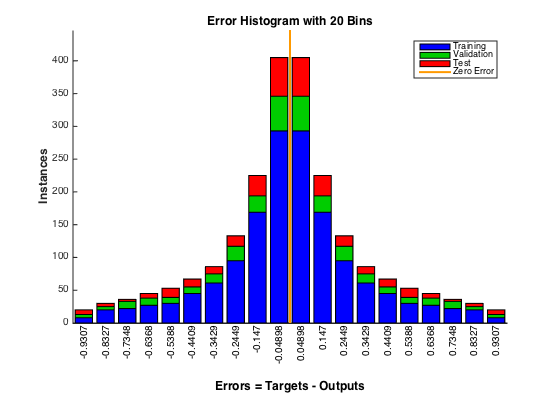
\includegraphics[width=1\linewidth]{../images-update/1-(4)-netural-error.png}
		\caption{netural-error}
		\label{fig:sub1}
	\end{subfigure}
	
	\begin{subfigure}{.5\textwidth}
		\centering
		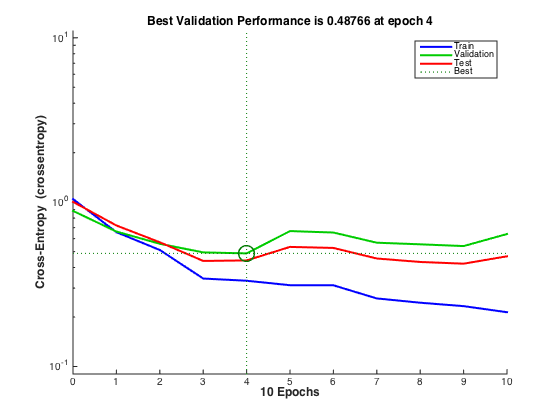
\includegraphics[width=1\linewidth]{../images-update/1-(4)-neural-perfomance.png}
		\caption{perfomance}
		\label{fig:sub1}
	\end{subfigure}
	%\caption{Data histograms before normalization.}
	%\label{fig:hist1}
	
	\begin{subfigure}{.5\textwidth}
		\centering
		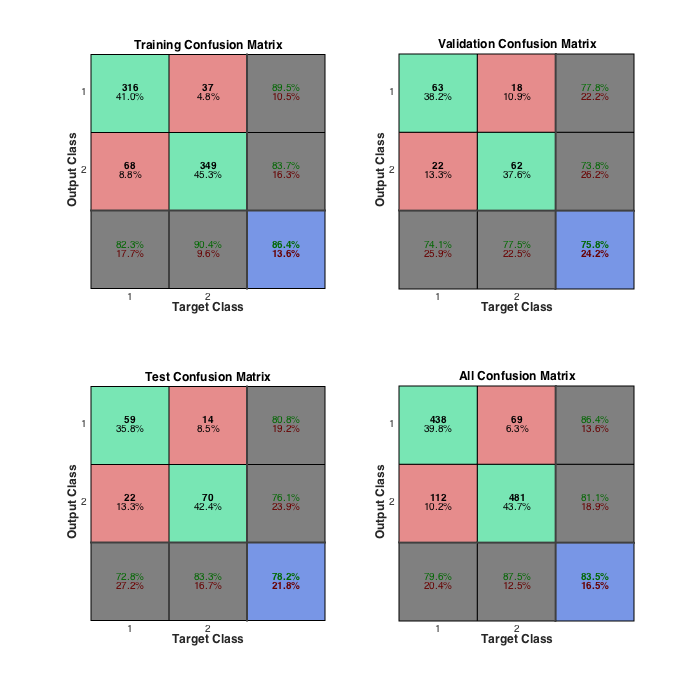
\includegraphics[width=1\linewidth]{../images-update/1-(4)-neural_confusion.png}
		\caption{neural-confusion}
		\label{fig:sub1}
	\end{subfigure}
	
	\begin{subfigure}{.5\textwidth}
		\centering
		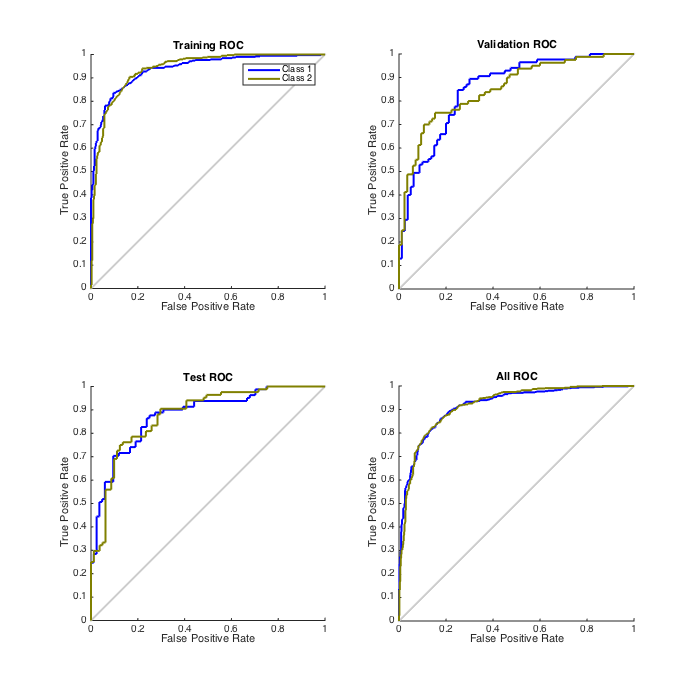
\includegraphics[width=1\linewidth]{../images-update/1-(4)-neural_receiver.png}
		\caption{neural-receiver}
		\label{fig:sub1}
	\end{subfigure}
	
	\begin{subfigure}{.5\textwidth}
		\centering
		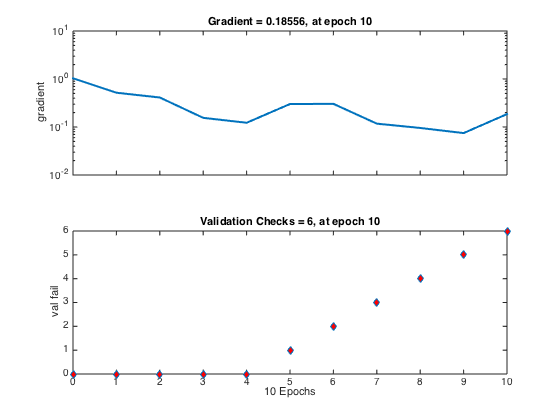
\includegraphics[width=1\linewidth]{../images-update/1-(4)-neural_gradient.png}
		\caption{neural-gradient}
		\label{fig:sub1}
	\end{subfigure}
	
\end{figure}
\begin{tabular}
	{l*{6}{c}r}   	& K-NN  & SVM & Naive Bayes & Decesion tree & Neural Network \\ \hline
	Accuracy & 74.4182 & 0 & 86.4864 & 92.9818 & 82.5773 \\ 
	std accuracy & 1.2322 & 0 & 0.6734 & 0.9843 & 1.7322 \\
	Precision & 0.9104 & 0 & 0.8603 &0.9391 & 0.8461\\
	std Precision & 0.028 & 0 & 0.0101 & 0.0146 & 0.0240\\
	recall & 0.5415 & 0 & 0.8810 & 0.9250 & 0.8089\\
	std recall & 0.0293 & 0 & 0.0104 & 0.0126 & 0.0330\\
	F-measure & 0.6782 & 0 & 0.8705 & 0.9319 & 0.8265 \\
	std F-measure & 0.0195 & 0 & 0.0060 & 0.0093 & 0.0186 \\
	Training time (S/Sample) & NA & 0 & 0.0093 & 0.00518 & 0.2698 \\
	Classification Time(Sample) & NA(?) & 0 & 0.0026 & 0.0104 & 0.0082 \\
\end{tabular}

\subsubsection{question 5}
5)Comment on the obtained results, what are the benefits and weaknesses of each method on this dataset. How could this analysis help to make the choice of the right method to use for a dataset of this type in the future?

For test accuracy, it could be reflected by accuracy, precision and f-measure. At the same time we could also combine the std to see the stable result.Precision is how useful the search results are, and recall is how complete the results are.high precision means that an algorithm returned substantially more relevant results than irrelevant, while high recall means that an algorithm returned most of the relevant results.Recall is defined as the number of relevant documents retrieved by a search divided by the total number of existing relevant documents, while precision is defined as the number of relevant documents retrieved by a search divided by the total number of documents retrieved by that search. For f-meansure, it considers both the precision p and the recall r of the test to compute the score: p is the number of correct positive results divided by the number of all positive results, and r is the number of correct positive results divided by the number of positive results that should have been returned. The F1 score can be interpreted as a weighted average of the precision and recall, where an F1 score reaches its best value at 1 and worst at 0.


From the above table, we could get the conclusion that Decision tree method could get the highest accuracy. The std accuracy is also has a relatively low level, so it means the average result is relatively stable. For the precision and std precision, all of the methods have a good performance, but maybe the best one is still the decision method.For recall and std recall, we could also get the conclusion that decision tree method and neural network have better perfomance, which means that the thue positive divided by the correct answer for both true positive and false negative is high. Similarly, the decision tree method also have the good performance for f-measure and std-measure.

For trainig time and classification time, since for K-NN, the algorithm always choose the k nearsest points, so there is no training time, and for classification time in K-NN, it should compare all test samples with test sampeles. For time percepective, naive bayes has the best perfomance. 

K-NN: Training a k-NN classifier simply consists of determining k and preprocessing documents. In fact, if we preselect a value for k and do not preprocess, then kNN requires no training at all. It means that for K-NN, there is no training process and for the classification process, compare the test sample with all of the samples, the time measure has been divided by all of samples.But the disadvantage of K-NN is that irrelevant dimensions could have bad influence a lot.

For SVM: For linear SVMs, at training time you must estimate the vector w and bias b by solving a quadratic problem, and at test time prediction is linear in the number of features and constant in the size of the training data. For kernel SVMs, at training time you must select the support vectors and at test time your complexity is linear on the number of the support vectors (which can be lower bounded by training set size * training set error rate) and linear on the number of features (since most kernels only compute a dos product; this will vary for graph kernels, string kernels, etc).So from the above the SVM maybe the time consuming most.SVMs contain an underlying optimization step that is solved heuristically, so for any actual algorithm that purports to solve SVMs, the answer is undefined. A number like O(n*n*n)is generally bandied around for implementations like libsvm, which means something like time/iteration * number of iterations (where numbr of  iterations is assumed to be constant)



Naïve Bayes Classifier: As we could conclude from the table that it is the most efficient method, linearly proportional to the time needed to just read in all the data.

Decision Trees: Decision trees are easy to use compared to other decision-making models, but preparing decision trees, especially large ones with many branches, are complex and time-consuming affairs.Computing probabilities of different possible branches, determining the best split of each node, and selecting optimal combining weights to prune algorithms contained in the decision tree are complicated tasks that require much expertise and experience.Decision trees moreover, examine only a single field at a time, leading to rectangular classification boxes. This may not correspond well with the actual distribution of records in the decision space.In reality, the complexity in creating large decision trees mandates people involved in preparing decision trees having advanced knowledge in quantitative and statistical analysis. This raises the possibility of having to train people to complete a complex decision tree analysis. The costs involved in such training makes decision tree analysis an expensive option, and remains a major reason why many companies do not adopt this model despite its many advantages. But the advantage of this method is it provide easy way to view illustrations.


Neural Networks: Since for each layer it could be lots of combination, and the number of layers are not a certain number for different situation, so this method could be time consuming.(not sure about this part analyse)



\section{Clustering Analysis (for dataset F)}
The data has already been normalized into the range of [-1, 1], the sample labels are used for the purpose of performance evaluation.
Apply PCA to reduce the dimension to be 4, and then conduct the following clustering analysis.
\subsection{question 1}
1) Perform hierarchical clustering using agglomerative algorithms:
a) Stop when the number of clusters is 10 (the same as the number of given classes). Compare the linkage methods of “single”, “complete”, and “ward (minimum variance algorithm)”. Evaluate the clustering results in terms of Separation-Index, Rand-Index, and F-measure. Compare the three linkage types and comment.

For clustering data into 10 classes, we could use the matlab library function “clusterdata”. Firstly, for separation-index, we should calculate the center of each cluster and calculate the square of each distance for each point with the center point. Later, we could use the result to divided by the total number of rows muliply the maximum distance for each cluster. And for rand-index, it should be calculated by (a+d)/M, here 'a' means TP and 'd' means FN, M means total number of comparation. For f-measure, we should firstly caluculate the number of objects in class j and cluster i, at the same time should also calulate the number of objects in class i as ni and number of objects in class j as nj. Later we could get the result of precision and recall. Lastly we could get the result using the function:   
F(i,j) = 2*precision(i,j)* recall(i,j)/(precision(i,j)+recall(i,j)).
For different algorithm, should use the function of 'single', 'complex' and 'ward'.




And according to the definition, we could get the conclusion that the result of separation-index is highly depending on the cluster result. Smaller separation-index means that every point in the cluster is close and as a result there could be more groups.
The result of rand-index and f-measure could have the similar trend for representing accuracy of the same cluster group, which is corresponding different with separation-index. It means that if there is a higher accuracy for cluster, the rand-index and f-measure could correspondingly higher, but it means larger size of cluster, as a result separation-index could be lower.



For separation-index there are two ways to calculte, one is for the maxium distance and another is for minimum distance. Below the first table shows the result for the maxmium distance and the second table shows the result for minimum distance. 
For maximum distance method:
For linkage method=single\\
Separation-Index=1.7540 \\
Rand-Index=0.1097\\
F-measure= 0.0962\\
For linkage method=complete\\
Separation-Index=0.6151 \\
Rand-Index=0.8184 \\
F-measure=0.2168\\
For linkage method=ward\\
Separation-Index=0.4937 \\
Rand-Index=0.8772 \\
F-measure= 0.2801 \\

For maximum distance method:
For linkage method=single\\
Separation-Index=? \\
Rand-Index=0.1097\\
F-measure= 0.0962\\
For linkage method=complete\\
Separation-Index=? \\
Rand-Index=0.8184 \\
F-measure=0.2168\\
For linkage method=ward\\
Separation-Index=? \\
Rand-Index=0.8772 \\
F-measure= 0.2801 \\


For separation-index, according to the function, we could get the conclution that when we choose the maximum method, the samller the value it is, the more densy it could be for a class. The trend should be different with rand-index and f-measure. So, the ward algorithm have the best result for the samllest separation-index and the largest rand-index and f-measure value. After we change the separation-index method for the maximum distance, it could be a slightly changed, but ward algorithm is still could be considered to be the best algorithm.

b) Fix the linkage type as “ward”, study the number of clusters from 2 to 15, increment by 1, what is the optimal number of clusters suggested by Separation- Index in this case?

After we run the 'ward' algorithm, and could the result for best cluster number is 15.

\subsection{question 2}
2) Cluster the data using k-means algorithm.
a) Run the algorithm for the number of clusters k from 2 to 15, increment by 1. Evaluate the clustering results in terms of Separation-Index, Rand-Index, and F-measure.

For calculation method of separation-index, rand-index and f-measure, they are similar with the above. The algorithm of k-means could be run by the function “kmeans”, and we could see the picture for 2-2-(a). We could see that both rand-index increase a lot with the increasing number of cluster, and f-measure increase a lot at the beginning and later a little bit decrease, but separation-index decrease.



The algorithm of k-means could be run by the function “kmeans”, and we could see the picture for 2-2-(a). We could see that both rand-index increase a lot with the increasing number of cluster, and f-measure increase a lot at the beginning and later a little bit decrease.



The reason why rand-index increase is because of the calculating function with the increasing number of cluster, it is closer to the right cluster way, but for the value of M it did not change, so it has an increasing trend. Similarly, f-measure also increase, for increasing number of clusters, it could reflect better accuracy. But for the separation-index, with the increasing number of cluster, the distance between different cluster could increase also, which could be a dominate part, so that we could see the trend is decreasing.

b) Plot these evaluation measures with respect to the number of clusters. What is the optimal number of clusters suggested by these indexes?

Combined with three methods, the best cluster number is 8, without too high separation-index or too low rand-index and f-measure.


\begin{figure}[p]
	\centering
	\begin{subfigure}{.5\textwidth}
		\centering
		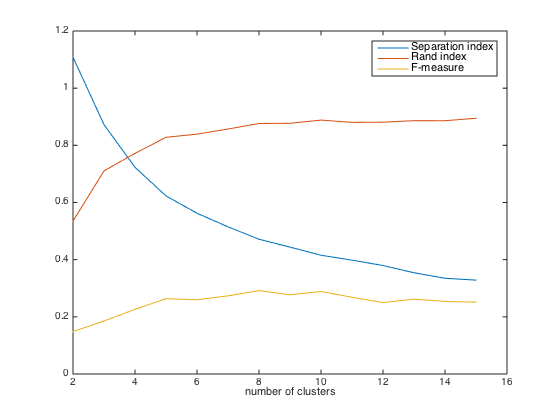
\includegraphics[width=1\linewidth]{../images-update/2-(2)-3.png}
		\caption{k-means algorithm}
		\label{fig:sub1}
	\end{subfigure}
	
	
	
\end{figure}



\subsection{question 3}

3) Cluster the data using fuzzy c-means algorithm, with number of clusters as 10, and the fuzzy parameter (the exponent for partition matrix) m = 2.

a) Plot the average cluster membership values for the samples of the digit ‘1’ and ‘3’; explore their overlaps with other clusters.

For the fuzzy c-means methods, we could use 'fcm' function directly, and label the result is same with digit '1' or '3', so that we could get the graph below.

\begin{figure}[p]
	\centering
	\begin{subfigure}{.5\textwidth}
		\centering
		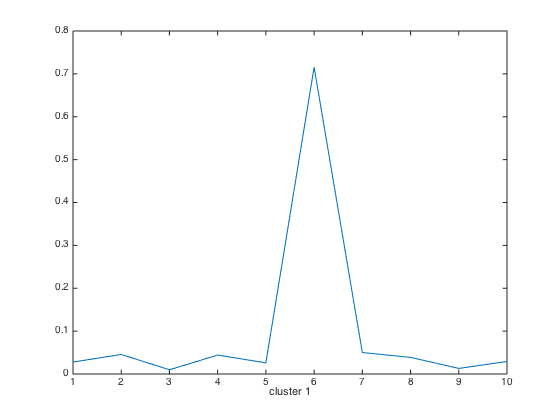
\includegraphics[width=1\linewidth]{../images-update/2-(3)-(a)-2.png}
		\caption{digit 1}
		\label{fig:sub1}
	\end{subfigure}
	
	\begin{subfigure}{.5\textwidth}
		\centering
		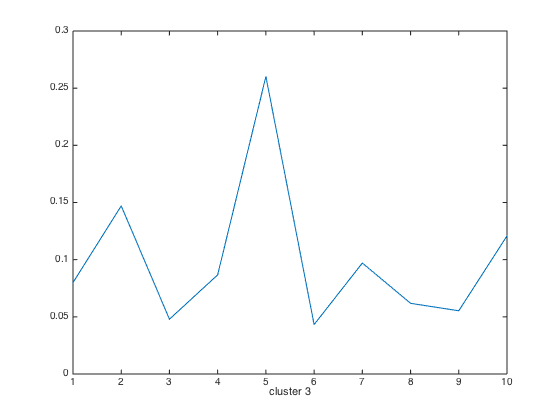
\includegraphics[width=1\linewidth]{../images-update/2-(3)-a-1.png}
		\caption{digit 3}
		\label{fig:sub1}
	\end{subfigure}
	
\end{figure}

From the graph, we could see that, for digit 1, it mainly in cluster 5 to 7, without too much overlapping with other groups. However, the result of digit 3 could be checked in different clusters, which means that there are more overlaps in cluster 3 but less in cluster 1.For the reason why there is less overlapping for digit 1 maybe for the hand writting dataset, the digit '1' is hard to make confusing with other digits unlike digit '3', 
 
b) If we produce hard clustering by making the max membership value of a sample to be one and the rest of its membership values zero, evaluate the clustering results. Comment on the obtained results.

In fuzzy clustering (also referred to as soft clustering), data elements can belong to more than one cluster, and associated with each element is a set of membership levels.But in hard clustering, data is divided into distinct clusters, where each data element belongs to exactly one cluster. For this question, we label the max member to be one group and the left one to be another group. 

For Fuzzy c-means\\
Separation-index=0.4454\\
Rand-Index=0.8905\\
F-measure=0.2844\\

For linkage method=single\\
Separation-Index=1.7540 \\
Rand-Index=0.1097\\
F-measure= 0.0962\\
For linkage method=complete\\
Separation-Index=0.6151 \\
Rand-Index=0.8184 \\
F-measure=0.2168\\
For linkage method=ward\\
Separation-Index=0.4937 \\
Rand-Index=0.8772 \\
F-measure= 0.2801 \\

So from the above, we could get the conclution that, fuzzy-c means has a better perfomance than other three methods.



\end{document}